\documentclass[../report.tex]{subfiles}
\begin{document}
\section{Phase 2 : Variables}
Cette section documente le travail réalisé pour atteindre les fonctionnalités de la phase 2 du projet. Ces fonctionnalités sont les mêmes que celles de la phase 1, mais avec en plus le support des variables dans les requêtes et dans les fichiers Prolog.
\subsection{Besoins}
Les besoins de cette phase sont les suivants :
\begin{itemize}
    \item Ajout du support des variables au parser
    \item Ajout d'une représentation en Java d'une variable Prolog
    \item Implémentation de l'unification
    \item Support de l'affichage des variables ayant conduit à un succès
\end{itemize}
\subsection{Plan}
En se basant sur l'état actuel du projet, on peut dresser le plan de réalisation suivant : modifier les composants existants pour intégrer les variables, en commençant par trouver une représentation en Java pour les variables et adapter le parser pour celles-ci, puis continuer en adaptant l'interpréteur et le noeud de résolution.
\subsection{Représentation des variables}
En se basant sur la structure décrite à la section \ref{subsec:prologRules}, on sait que les variables sont également des termes. Les variables logiques ont cependant une particularité : elles représentent des inconnues, et peuvent donc prendre une valeur si cela s'avère nécessaire pour s'unifier. En conséquence, pour modéliser ce comportement, elles peuvent se retrouver liées à un autre terme (qui peut être une autre variable). La figure \ref{fig:part2classdiagram} montre une représentation possible des éléments Prolog en Java, avec les variables.
\begin{figure}[h]
    \centering
    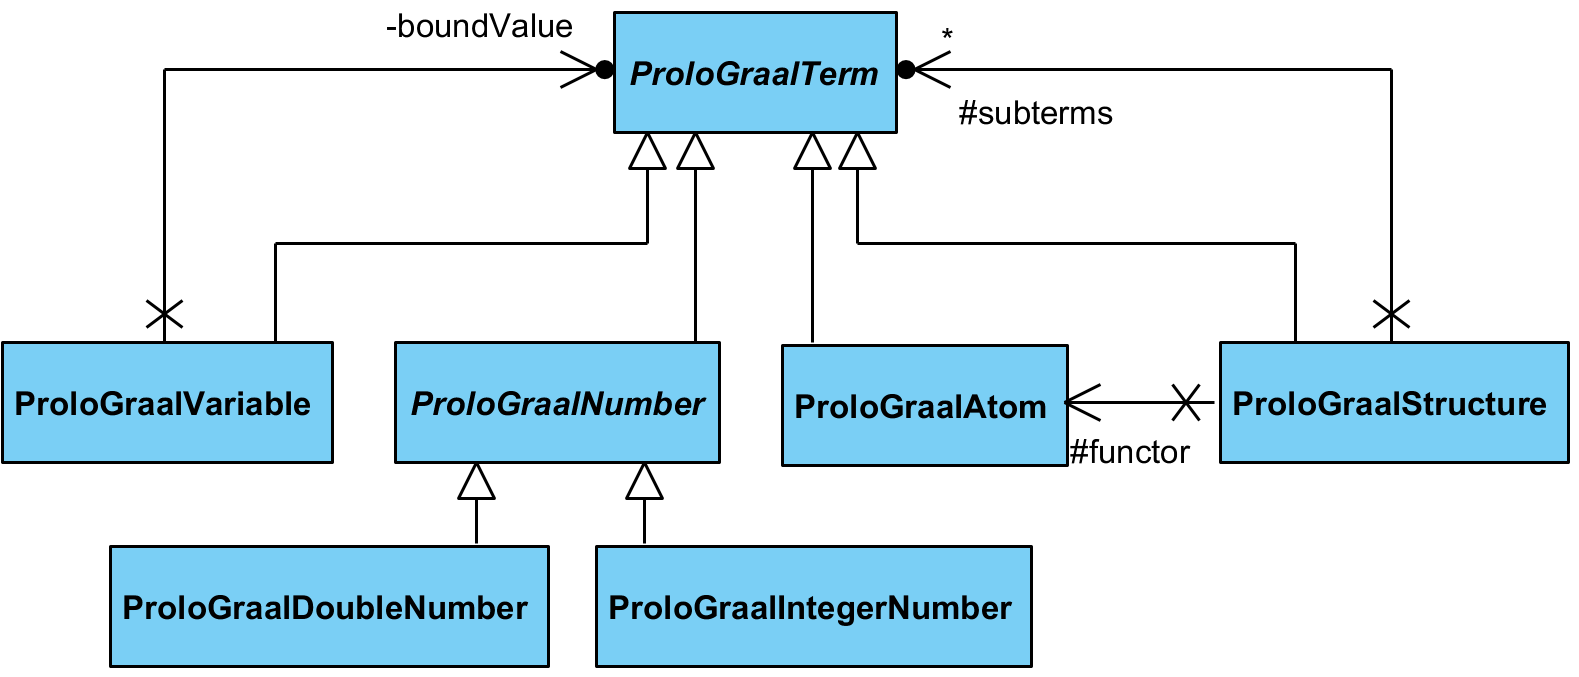
\includegraphics[width=\textwidth]{part2classdiagram.png}
    \caption{Diagramme de classes des éléments Prolog en Java, variables incluses}
    \label{fig:part2classdiagram}
\end{figure}
\subsection{Adaptation du parser}
Pour adapter le parser afin que celui-ci intègre les variables, trois éléments sont à modifier, dans l'ordre :
\begin{enumerate}
    \item Le lexer dans la grammaire ANTLR, pour qu'il comprenne que les chaînes commençant par une majuscule(ou un tiret bas) sont des variables
    \item Le parser dans la grammaire ANTLR, pour qu'il comprenne qu'une variable est composée de l'unité "variable" du lexer
    \item Le listener, pour créer les représentations Java des variables
\end{enumerate}
\subsubsection{Lexer}
Dans la grammaire ANTLR, on rajoute un nouvel élément représentant une variable au lexer. Une variable commence soit par une majuscule, soit par un tiret bas, suivi d'un certain nombre de caractères.
\begin{minted}[breaklines]{ANTLR}
VARIABLE : ((UPPERCASE | UNDERSCORE) (LOWERCASE | UPPERCASE | DIGITS | UNDERSCORE)*);
\end{minted}
\subsubsection{Parser}
Pour la partie parser, on doit rajouter dans la grammaire ANTLR deux choses : un terminal composé de l'élément du lexer "variable", et dire qu'un terme peut être aussi une variable.
\begin{minted}{ANTLR}
variable :
VARIABLE
;
term :
functor ('(' term (',' term)* ')') |
atom | 
number |
variable
;
\end{minted}
\subsubsection{Listener}\label{subsubsec:phase2listener}
Pour le listener, on pourrait penser qu'il suffit de créer une nouvelle variable avec le bon nom et de l'ajouter à la structure courante. Mais cette approche sera rapidement victime d'un problème : si la même variable est référencée plusieurs fois dans la même structure (exemple : \mintinline{Prolog}{fait(X, X).}), alors deux instances indépendantes seront créées, ce qui pose problème au moment où une de ces variables prendra une valeur, car l'autre doit obligatoirement prendre la même valeur pour que le comportement soit correct, ce qui nécessiterait de gérer la synchronisation manuellement.

Pour pallier ce problème, on va profiter du mécanisme de référence de variables en Java. L'algorithme imaginé est le suivant\footnote{une version améliorée de cet algorithme basée sur des "Map" est présentée plus tard à la section \ref{subsubsec:phase3listener}} : on tient à jour une liste des variables de la structure courante. Quand on rencontre une variable, on vérifie si elle existe déjà dans cette liste. Si oui, alors on la récupère et on place sa référence dans la structure courante. Si non, on la crée et on l'ajoute à la structure courante et à sa liste de variables.

Dans l'implémentation, la liste de variables est en fait une liste de listes : chaque entrée correspond à une entrée dans la liste des clauses, et pour chaque clause on peut avoir un certain nombre de variables :
\begin{minted}{Java}
private List<ProloGraalTerm<?>> clauses;
private List<List<ProloGraalVariable>> variablesForEachClause;
\end{minted}
Dans la méthode \mintinline{Java}{enterVariable}, on va réaliser l'algorithme présenté précédemment. On commence par créer une variable représentant celle que l'on vient de rencontrer dans le code source, pour pouvoir la comparer avec les existantes. On récupère également la liste des variables de la clause courante :
\begin{minted}[breaklines]{Java}
ProloGraalVariable var = new ProloGraalVariable(ctx.getText());
List<ProloGraalVariable> variablesForThisClause = variablesForEachClause.get(variablesForEachClause.size() - 1);
\end{minted}
On va ensuite chercher dans la liste des variables pour voir si la variable actuellement traitée est nouvelle ou non, et l'ajouter si nécessaire. À l'aide de la \textit{Stream API} de Java et de quelques astuces, on peut écrire cette opération de manière très concise et élégante :
\begin{minted}[breaklines]{Java}
final ProloGraalVariable var2 = var;
// if the variable was previsouly encountered in this scope, do not add a new one
var = variablesForThisClause.stream().filter(x -> x.equals(var2)).findFirst().orElseGet(() -> {
    variablesForThisClause.add(var2);
    return var2;
});
add(var);
\end{minted}
\subsubsection{Retour du parser}\label{subsubsec:phase2parser}
Pour simplifier les opérations sur les variables, comme par exemple la remise à zéro après la résolution d'un but, il serait intéressant de conserver directement la liste des variables et de la rendre disponible pendant la résolution. On va donc créer une nouvelle classe \mintinline{Java}{ProloGraalParseResult}, dont l'unique but est de stocker à la fois une référence vers la liste des clauses, et une référence vers la liste de listes des variables. Le retour final du parser est donc le suivant : 
\begin{minted}[breaklines]{Java}
return new ProloGraalParseResult(listener.getClauses(), listener.getVariables());
\end{minted}
Dans la classe \mintinline{Java}{ProloGraalLanguage}, on va donc récupérer cet objet et le transmettre au \mintinline{Java}{ProloGraalEvalRootNode}, qui se charge d'enregister la référence vers les clauses et celle vers les variables dans le contexte. Ces deux éléments sont donc accessibles pour notre \mintinline{Java}{ResolverNode}.
\subsection{Adaptation du noeud de résolution}
Vu que nous avons maintenant des variables, il ne suffit plus de chercher les termes étant exactement égaux au but courant; il faut trouver tous les termes \textit{unifiables} avec le but courant. L'algorithme est le suivant : pour chacun des termes du contexte (nos faits), on regarde s'il est unifiable avec le but. Si oui, on l'ajoute à la liste des succès. Il faut ensuite défaire tous les changements que le processus d'unification aurait pu engendrer, en réinitialisant les variables du but et de chaque fait. Cet algorithme se code de cette manière :
\begin{minted}[breaklines]{Java}
for(int i = 0; i < terms.size(); i++) {
    ProloGraalTerm<?> clause = terms.get(i);
    if(clause.isUnifiable(goal)) {
        System.out.println("Success with clause : " + clause.toString());
        successes.add(new ProloGraalSuccess(clause, variables.get(i)));
    }
    variables.get(i).forEach(ProloGraalVariable::unbind);
    goalVariables.forEach(ProloGraalVariable::unbind);
}
\end{minted}
Reste à définir le processus d'unification et sa logique propre à chaque type de terme.
\subsection{L'unification}
Le processus d'unification dépend du type du terme en question. Pour représenter ce comportement, la surcharge de fonctions avec notre structure présentée à la figure \ref{fig:part2classdiagram} se prête particulièrement bien. On déclare donc notre méthode d'unification de la manière suivante, dans notre classe mère\footnote{Son nom n'est pas particulièrement bien choisi, vu qu'elle peut modifier les objets pour les rendre unifiables. Elle sera plus tard renommée en simplement \texttt{unify}.} :
\begin{minted}{Java}
public abstract boolean isUnifiable(ProloGraalTerm<?> other);
\end{minted}
\subsubsection{Principe général}
Le principe général de l'unification mis en place est que chaque type de terme est responsable de l'unification avec un élément de son propre type. Mais si l'autre élément est une variable, alors la logique est déléguée à la variable. L'unification étant bidirectionnelle, le résultat ne change pas, mais l'implémentation est simplifiée avec toute la logique inter-types présente uniquement dans le code des variables.
\subsubsection{Atomes et nombres}
Pour les atomes et les nombres, le processus est très simple : pour que l'unification soit possible, il faut que l'autre élément soit du même type, avec la même valeur, ou qu'il soit une variable :
\begin{minted}{Java}
@Override
public boolean isUnifiable(ProloGraalTerm<?> other) {
    if(this.equals(other)) {
        return true;
    } else if(other instanceof ProloGraalVariable) {
        return ((ProloGraalVariable)other).isUnifiable(this);
    }
    return false;
}
\end{minted}
On remarque également le principe expliqué précédemment de déléguation de la logique à la variable.
\subsubsection{Structures}
Pour les structures, il faut que les deux aient le même foncteur et la même arité, et il faut que chaque sous-terme s'unifie avec son correspondant direct (le premier sous-terme de la première structure doit s'unifier avec le premier sous-terme de la seconde structure). L'unification est donc un succès uniquement si tous les sous-termes sont unifiables. Même si l'on peut potentiellement modifier les sous-termes, les opérations seront quand même correctement défaites en cas d'échec, car toutes les variables sont dans la même liste, même celles qui sont imbriquées (cf. \ref{subsubsec:phase2listener}). 
\begin{minted}[breaklines]{Java}
@Override
public boolean isUnifiable(ProloGraalTerm<?> other) {
    if(this.equals(other)) {
        for(int i = 0; i < this.arity; i++) {
            if(!this.subterms.get(i)
                .isUnifiable(((ProloGraalStructure)other).subterms.get(i))) {
                return false;
            }
        }
        return true;
    } else if(other instanceof ProloGraalVariable) {
        return ((ProloGraalVariable)other).isUnifiable(this);
    }
    return false;
}
\end{minted}
\subsubsection{Variables}
Pour les variables, le processus se décline en deux variantes :
\begin{itemize}
    \item Si la variable est déjà liée à une autre valeur, alors on essaie d'unifier cette valeur avec l'autre élément.
    \item Si la variable n'est pas déjà liée, alors on la lie avec l'autre élément et l'unification est un succès.
\end{itemize}
Il y a également tous les cas spéciaux dans le cas où l'autre élément est également une variable, et les problèmes engendrés par les références cycliques. Ces problèmes sont analysés et partiellement résolus plus tard dans la section \ref{subsec:unificationfixes}. Mais pour l'instant, on en reste à une implémentation basique :
\begin{minted}[breaklines]{Java}
@Override
public boolean isUnifiable(ProloGraalTerm<?> other) {
    // can always unify to itself
    if(other instanceof ProloGraalVariable && (ProloGraalVariable)other == this)
        return true;
    if(this.isBound) {
        if(other instanceof ProloGraalVariable) {
            ProloGraalVariable otherVar = (ProloGraalVariable)other;
            if(otherVar.isBound) {
                return this.boundValue.isUnifiable(otherVar.boundValue);
            } else {
                otherVar.bind(this);
                return true;
            }
        } else {
            return this.boundValue.isUnifiable(other);
        }
    } else {
        this.bind(other);
        return true;
    }
}
\end{minted}
Pour aider à ce processus, une méthode permettant de lier la variable à un élément a été implémentée. Cette méthode pratique également un test très simple\footnote{et très incomplet...} pour tenter de détecter les cas cycliques :
\begin{minted}{Java}
public void bind(ProloGraalTerm<?> other) {
    if(other instanceof ProloGraalVariable) {
        ProloGraalVariable otherVar = (ProloGraalVariable)other;
        if(otherVar.isBound && otherVar.boundValue == this) {
            return;
        }
    }
    this.isBound = true;
    this.boundValue = other;
    System.out.println(name + " = " + other);
}
\end{minted}
Ainsi que sa correspondante permettant de défaire la liaison :
\begin{minted}{Java}
public void unbind() {
    this.isBound = false;
    this.boundValue = null;
}
\end{minted}
\subsection{Affichage des résultats}
Pour le retour des résultats depuis le noeud de résolution et ensuite leur affichage dans l'interpréteur, l'état des variables du but est sauvegardé à chaque succès. Pour cela, une méthode de copie de l'état actuel d'une variable est implémentée :
\begin{minted}{Java}
@Override
public ProloGraalVariable copy() {
    ProloGraalVariable var = new ProloGraalVariable(this.name);
    var.isBound = this.isBound;
    if(this.isBound) {
        var.boundValue = this.boundValue.copy();
    }
    return var;
}
\end{minted}
Ces succès se retrouvent encapsulés dans une liste de \mintinline{Java}{ProloGraalSuccess} qui est remontée au noeud d'interprétation. Celui-ci se charge de lire l'état des variables pour chaque succès et de l'afficher :
\begin{minted}[breaklines]{Java}
ProloGraalBoolean callResult = (ProloGraalBoolean) Truffle.getRuntime().createCallTarget(context.getResolverNode()).call(runtime);
if(callResult.asBoolean()) {
    ProloGraalSuccess success = (ProloGraalSuccess)callResult;
    if(success.getSuccesses().size() > 0) {
        for(ProloGraalSuccess succ : success.getSuccesses()) {
            succ.getVariables().forEach(x -> {
                if(x.isBound())
                    writer.println(x);
            });
        }
    }
}
writer.println(callResult);
\end{minted}
\subsection{Synthèse}
La phase 2 est maintenant terminée. Il reste de nombreux bugs (dont beaucoup qui seront découverts par la suite), mais l'objectif de cette phase est atteint : nous avons une représentation des variables Prolog en Java, ainsi qu'un mécanisme d'unification sommaire.
\end{document}